\chapter{LE2ML: un \textit{workbench} modulaire pour l'apprentissage machine}
\label{chap:6}

\section{Introduction}

Grâce aux chapitres précédents, il a été montré, dans un premier temps, que les \textit{wearable devices} sont de plus en plus utilisés dans le processus de reconnaissance d'activités au sein des habitats intelligents. Aussi, ces dispositifs ont également été employés dans l'objectif de répondre à plusieurs autres problématiques relatives à l'assistance des résidents de ces habitats, au sens large. Néanmoins, l'engouement croissant pour les \textit{wearable devices} a permis d'identifier plusieurs problématiques quant à leur utilisation dans ce contexte de recherche particulier. En effet, il a été évalué que la plupart des différentes architectures d'habitats intelligents qui ont été proposées n'ont pas été conçues dans une optique évolutive. Ainsi, celles-ci ne permettent pas d'y intégrer de manière rapide et efficace de nouveaux capteurs, comme les \textit{wearable devices}, ou de nouveaux composants logiciels pour réaliser le processus de reconnaissance d'activités et l'assistance aux résidents.

Pour ce travail, l'intégration des \textit{wearable devices} dans les architectures de maisons intelligentes s'est concentrée avant tout sur un aspect logiciel plutôt que matériel des différentes méthodes de reconnaissances que ces dispositifs proposent. En effet, tout comme pour la reconnaissance d'activités réalisée de manière classique, c'est-à-dire, en exploitant les capteurs et effecteurs statiques présents dans l'habitat, les différents processus proposés par les dispositifs sont, dans une vaste majorité des cas, encapsulés au sein d'un unique composant logiciel immuable. De la même manière, la réutilisation de mécanismes communs, le déploiement de ces méthodes et leur modification demeurent alors des tâches complexes à mettre en \oe{}uvre.

Malgré cela, certains travaux ont fait mention de l'emploi d'un \textit{workbench} d'apprentissage machine afin de traiter les données produites par les \textit{wearable devices} et effectuer la reconnaissance d'activité \citep{Chapron2018}. D'un point de vue académique, ces outils ne sont pas nouveaux et ils permettent un prototypage rapide, la visualisation des données ainsi qu'une meilleure reproductibilité des méthodes expérimentales et une meilleure réutilisation des composants logiciels \citep{Holmes1994,Langlois2008}. À titre d'exemple, l'outil le plus connu et le plus répandu dans la littérature est \acs{WEKA}. Il s'agit d'un \textit{workbench} open source développé en Java qui supporte un grand nombre d'algorithmes d'apprentissage machine supervisés et non supervisés \citep{Witten2016}. Celui-ci a été utilisé en tant que librairie dans la méthode de reconnaissance des types de sols présentée au chapitre \ref{chap:4}. Néanmoins, bien que ce \textit{workbench} offre un large éventail d'options, son utilisation reste relativement gourmande en termes d'utilisation des ressources de calcul et de mémoire. De plus, les fonctionnalités offertes par cet outil demeurent particulièrement contraignantes à étendre et de par sa conception, il n'est pas particulièrement adapté pour être utilisé dans l'architecture d'habitats intelligents distribuée qui a été introduite dans le chapitre précédent. Par ailleurs, avec la tendance qui entoure actuellement l'intelligence artificielle, ce type d'outil devient de plus en plus populaire depuis que des fournisseurs de \textit{cloud} publics, tels qu'\textit{Amazon AWS}, \textit{Google Cloud Plateform} et \textit{Microsoft Azure} ont introduit des versions grand public de ces applications. Comme elles font partie de la vaste liste de services payants proposés par chaque fournisseur, les \textit{workbench} d'apprentissage machine peuvent bénéficier de l'évolutivité qu'offre le \textit{cloud}. Cependant, comme ils sont considérés comme des services d'usage général, les mécanismes internes des techniques d'apprentissage machine ont été complètement occultés afin de les rendre accessibles à tous.

Ainsi, ce dernier travail présente \acs{LE2ML} (\acl{LE2ML}), un nouveau type de \textit{workbench} pour l'apprentissage machine qui repose sur l'utilisation de microservices. De la même manière que pour l'implémentation de l'architecture proposée, cette conception logicielle a été choisie, car la technologie des microservices permet une meilleure évolutivité, des déploiements plus sûrs et plus rapides ainsi qu'une meilleure isolation des pannes \citep{Dragoni2017}. Cependant, l'avantage principal d'une telle conception concerne l'aspect modulaire que permettent les microservices. Ainsi, ce \textit{workbench} demeure un outil agnostique tant en termes de langages de programmation que de plateformes supportées qui peut être déployé dans n'importe quel environnement, et ce, sans aucune contrainte complexe.

La suite de ce chapitre comporte une première section qui propose un état de l'art en matière de \textit{workbench} pour l'apprentissage machine, car ceux-ci ont joué, depuis plusieurs années, un rôle important dans différents champs de recherche. Ensuite, la section suivante introduit \acs{LE2ML}, le \textit{workbench} proposé et une expérimentation pour évaluer son fonctionnement et valider les résultats attendus est décrite dans une troisième section. Finalement, dans une dernière partie, ce chapitre dresse une conclusion quant à ce dernier travail.

\section{État de l'art}

Selon \cite{Langlois2008}, un \textit{workbench} d'apprentissage machine est un outil qui fourni une interface unifiée qui permet d'exploiter un certain nombre d'algorithmes d'apprentissage dans le but de traiter différents problèmes que ces méthodes peuvent potentiellement résoudre. Ainsi, au cours des dernières années, plusieurs de ces outils ont été développés et exploités dans divers domaines de recherche tels que la bio-informatique \citep{Larranaga2006}, la cybersécurité \citep{Handa2019}, la santé \citep{Rajkomar2019}, et plus particulièrement pour la reconnaissance d'activité à l'intérieur des habitats intelligents \citep{Ramirez-Prado2019}. Cette section décrit donc trois de ces outils d'apprentissage machine open-source qui sont parmi les plus utilisés dans la littérature. Ceci dans l'objectif principal d'identifier le besoin qui a motivé l'introduction de \acs{LE2ML}.

\subsection{WEKA}

\acs{WEKA} est un constitue un ensemble d'algorithmes d'apprentissage machine développé en Java qui a été introduit en 1994 principalement pour faciliter les tâches de forage de données (\textit{data mining}). Plus précisément, cet outil contient plusieurs fonctionnalités qui permettent d'effectuer du prétraitement de données, de la classification, de la régression, du \textit{clustering}, des règles d'association, de l'apprentissage profond et de la visualisation. Bien que \acs{WEKA} suggère son propre format de fichier natif (\acl{ARFF} ou \acs{ARFF}), il supporte également les fichiers \acs{CSV}, les fichiers Matlab ainsi que la connectivité à plusieurs bases de données \textit{via} \ac{JDBC}. En ce qui concerne le prétraitement des données, \acs{WEKA} propose un grand nombre de méthodes allant de la simple suppression d'attributs pour les ensembles de données à des opérations avancées comme l'analyse par composantes principales (\acs{PCA}).

Dans sa première version, \acs{WEKA} était uniquement exploitable au travers d'une interface en ligne de commande (\acs{CLI}). Aujourd'hui, bien qu'il soit toujours possible d'utiliser la \acs{CLI}, cet outil offre la possibilité d'être inclus en tant que dépendance d'un projet Java ou \textsf{R} \citep{Hornik2009}. De plus, il peut surtout être utilisé à travers plusieurs types d'interfaces graphiques. Dans un premier temps, la première possibilité demeure l'\emph{explorer}, où l'utilisateur peut mettre en place rapidement des techniques de manipulation des données (filtrage, classification, \textit{clustering} et visualisation), sans avoir besoin d'écrire de code. Dans un second temps, \acs{WEKA} propose une interface propre aux expérimentations : l'\emph{experimenter}. Il s'agit d'un outil permettant d'exécuter en parallèle, c'est-à-dire, selon différents processus sur une même machine ou sur différents ordinateurs d'un réseau, plusieurs expériences d'apprentissage machine afin d'évaluer les méthodes de classification et de régression. La troisième interface proposée par \acs{WEKA}, appelée \emph{knowledge flow}, offre la possibilité de réaliser les mêmes tâches qu'avec l'interface \emph{explorer}. Néanmoins, celles-ci sont représentées sous forme de blocs qui doivent être manipulés pour construire un processus de flux opérationnel (\textit{workflow}) comme le montre la figure \ref{fig:weka}. Cette dernière illustre un exemple d'utilisation de l'interface \emph{knowledge flow} pour un processus de classification sur les données du jeu de données iris \citep{Asuncion2007}. Dans cet exemple, l'algorithme \acs{KNN}, configuré avec $k=1$ voisin a été utilisé et la performance de la classification a été évaluée selon la technique de la séparation en $80/20$, c'est-à-dire, $80\%$ des données sont utilisées pour la phase d'entrainement, tandis que les $20\%$ restants sont exploités lors de la phase de reconnaissance.

\begin{figure}[H]
	\centering
	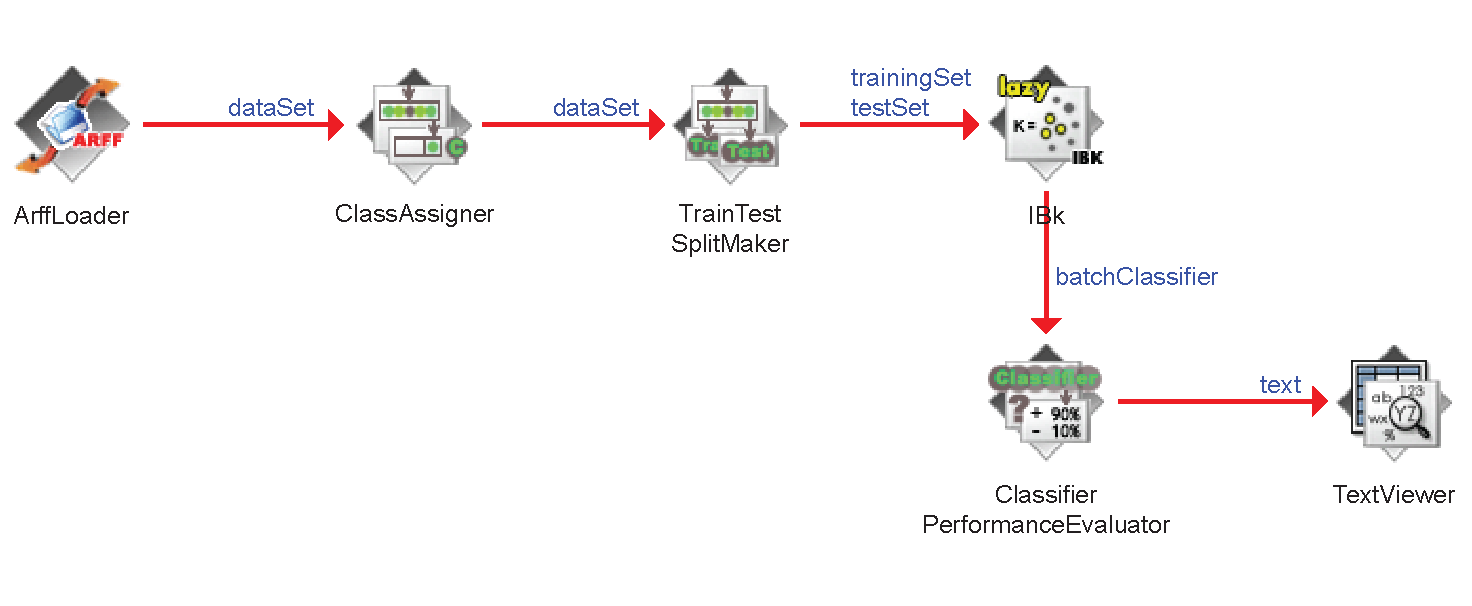
\includegraphics[width=.9\linewidth]{chapter6/weka.pdf}
        \caption{Exemple de l'interface \textit{knowledge flow} de \acs{WEKA} qui décrit un processus de classification sur le jeu de données iris avec l'algorithme \acs{KNN} où $k=1$ voisin et évaluée selon la technique de la séparation $80/20$.}
	\label{fig:weka}
\end{figure}

\acs{WEKA} est probablement le \textit{workbench} d'apprentissage machine le plus connu et le plus utilisé puisqu'il s'agit d'un outil portable \citep{Bouckaert2010} offrant un large éventail de possibilités pour réaliser facilement des processus liés à l'apprentissage machine. Cependant, cet outil présente plusieurs inconvénients. Premièrement, comme il est écrit en Java et qu'il repose sur une ancienne base de code, sa capacité à traiter une grande quantité de données et la rapidité des différentes opérations sont profondément affectées par une consommation importante de ressources. Plus récemment, un gestionnaire de paquets a été introduit afin de permettre à des développeurs tiers d'étendre les fonctionnalités de base du \textit{workbench} \citep{Hall2009}. Néanmoins, bien que ces nouvelles fonctionnalités ont permis à \acs{WEKA} de devenir plus flexible, le développement de ces paquets n'est possible qu'en Java et ceux-ci doivent respecter les contraintes d'intégration dans l'outil.

\subsection{RapidMiner}

RapidMiner, également connu sous le nom de \acs{YALE} (\acl{YALE}) \citep{Ritthoo2003,Hofmann2014}, a été développé à partir de 2001 puis rebaptisé en RapidMiner en 2007.  De la même manière que \acs{WEKA}, RapidMiner propose un environnement qui repose sur du code Java pour mettre en \oe{}uvre des techniques d'apprentissage machine. Cependant, contrairement à \acs{WEKA}, cet outil n'offre qu'une seule interface qui permet de définir des flux opérationnels à la façon de l'interface \textit{knowledge flow}. En effet, ces processus sont décrits à partir de blocs élémentaires appelés opérateurs. Il est alors possible pour l'utilisateur de composer une chaîne d'opérateurs en plaçant ces blocs sur un canevas et en câblant leurs ports d'entrée et de sortie, comme le montre la figure \ref{fig:rapid_miner}. Bien que \acs{WEKA} soit intégré dans RapidMiner en tant que dépendance utilisée pour plusieurs blocs, la majorité d'entre eux permettent d'étendre nombreux aspects de l'apprentissage machine qui ne sont pas nécessairement couverts par \acs{WEKA}.

Par ailleurs, RapidMiner inclut également la possibilité d'ajouter des paquets développés par des tiers afin d'améliorer ses capacités initiales. De plus, il permet l'utilisation d'un bloc de script où il est possible d'écrire du code en syntaxe Java ou Groovy. En ce sens, RapidMiner apparait tout aussi flexible que \acs{WEKA}. Cependant, puisqu'il repose sur une conception logicielle comparable et un langage de programmation de base identique, ce \textit{workbench} souffre des mêmes inconvénients. En outre, il est possible de dire que RapidMiner ne convient pas au déploiement d'applications expérimentales dans un contexte de recherche, car il ne dispose pas d'interface en ligne de commande et il n'est pas possible de l'utiliser comme une librairie dans une application.

\begin{figure}[H]
	\centering
	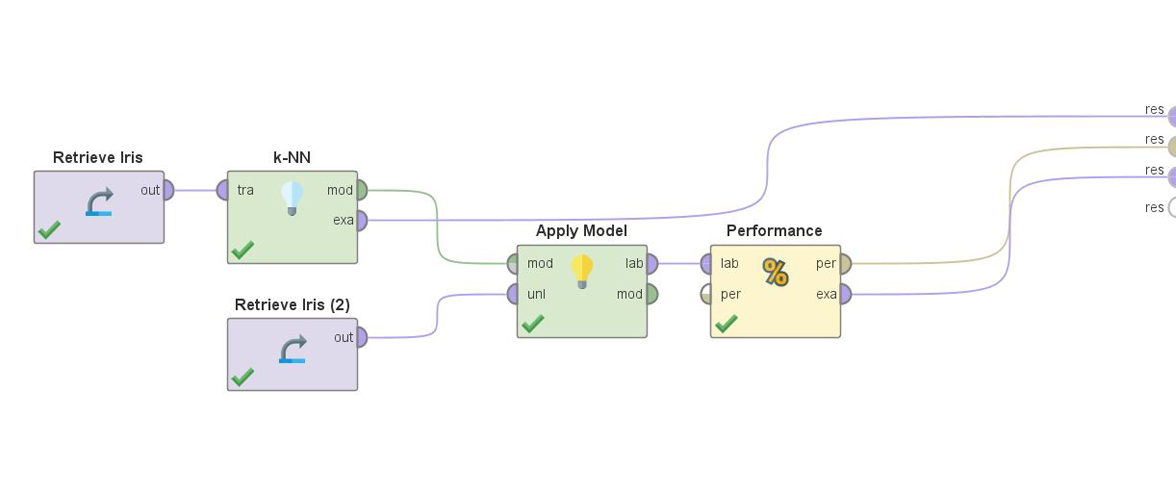
\includegraphics[width=.9\linewidth]{chapter6/rapid_miner.jpg}
        \caption{Exemple de chaîne d'opérateurs dans l'outil RapidMiner qui décrit un processus de classification sur le jeu de données iris avec l'algorithme \acs{KNN} où $k=1$ voisin et évaluée selon la technique de la séparation $80/20$.}
	\label{fig:rapid_miner}
\end{figure}

\subsection{Orange}

Orange est le dernier \textit{workbench} d'apprentissage machine, parmi les plus mentionnés dans la littérature, qui est présenté dans ce chapitre. Introduit en 1997, les fonctionnalités de base de cet outil ont été initialement conçues en \verb!C++! et sa couche logicielle supérieure (c'est-à-dire les modules et l'interface graphique) était développée en Python \citep{Demsar2004,Demsar2013}. Cependant, depuis 2015, Orange a été entièrement redéveloppé. L'ancien noyau \verb!C++! a été remplacé entièrement par du code Python et l'interface graphique a également été revue. De la même manière que \acs{WEKA}, Orange offre la possibilité soit d'être importé en tant que librairie dans un script Python, soit d'être utilisé comme outil à part entière grâce à interface graphique également basée sur l'utilisation de composants. En effet, comme le montre la figure \ref{fig:orange}, Orange permet également de manipuler des \emph{widgets} disposés sur un canevas qui, une fois reliés entre eux, permettent de définir un \emph{schéma} qui représente le flux opérationnel du processus d'apprentissage machine à réaliser. En outre, ce \textit{workbench} offre également la possibilité d'importer des \emph{widgets} personnalisés par l'intermédiaire d'un gestionnaire de paquets.

\begin{figure}[H]
	\centering
	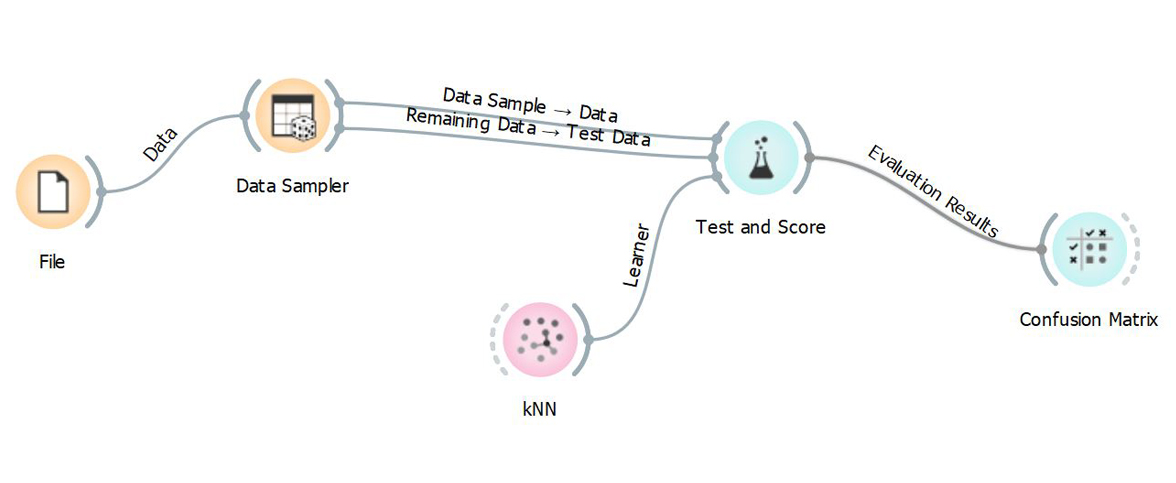
\includegraphics[width=.9\linewidth]{chapter6/orange.jpg}
        \caption{Exemple d'un \emph{schéma} dans Orange qui décrit un processus de classification sur le jeu de données iris avec l'algorithme \acs{KNN} où $k=1$ voisin et évaluée selon la technique de la séparation $80/20$.}
	\label{fig:orange}
\end{figure}

De la même manière que WEKA, puisqu'une intégration dans un programme Python est possible, Orange semble être tout autant susceptible d'être employé dans la conception d'applications académiques. De plus, étant donné que la version la plus récente d'Orange (Orange3) repose sur plusieurs outils modernes tels que NumPy\footnote{\url{https://numpy.org}}, SciPy\footnote{\url{https://www.scipy.org}} et scikit-learn\footnote{\url{https://scikit-learn.org}}, les possibilités de créer des widgets personnalisés sont illimitées. Par ailleurs, l'exécution d'un processus de classification réalisé avec Orange a montré une consommation de ressources (temps calcul et utilisation mémoire) plus raisonnable que pour le même processus effectué avec \acs{WEKA}. En revanche, les recommandations fournies qui documentent la conception de widgets personnalisés ne sont pas triviales et se limitent à du code Python.

\section{Solution proposée}

Dans la section précédente, les trois principaux \textit{workbench} d'apprentissage machine ont été présentés dans le but de déterminer les problématiques de chacune de ces solutions. Ainsi, il est apparu que tous ces outils présentent le même principal inconvénient, c'est-à-dire, une forte dépendance à leur contexte d'utilisation. En effet, toutes permettent d'intégrer des composants logiciels personnalisés, néanmoins ceux-ci doivent être conçus pour répondre aux exigences de l'outil pour lequel ils sont développés. De plus, dans un contexte de recherche académique, ces paquets additionnels peuvent devenir difficiles à maintenir. En effet, ils doivent être installés manuellement sur chacun des dispositifs qui composent l'environnement (\textit{p. ex.} ordinateurs ou serveurs), ce qui provoque indubitablement des problèmes de déploiement et de réutilisation de ces composants logiciels.

\begin{figure}[H]
	\centering
	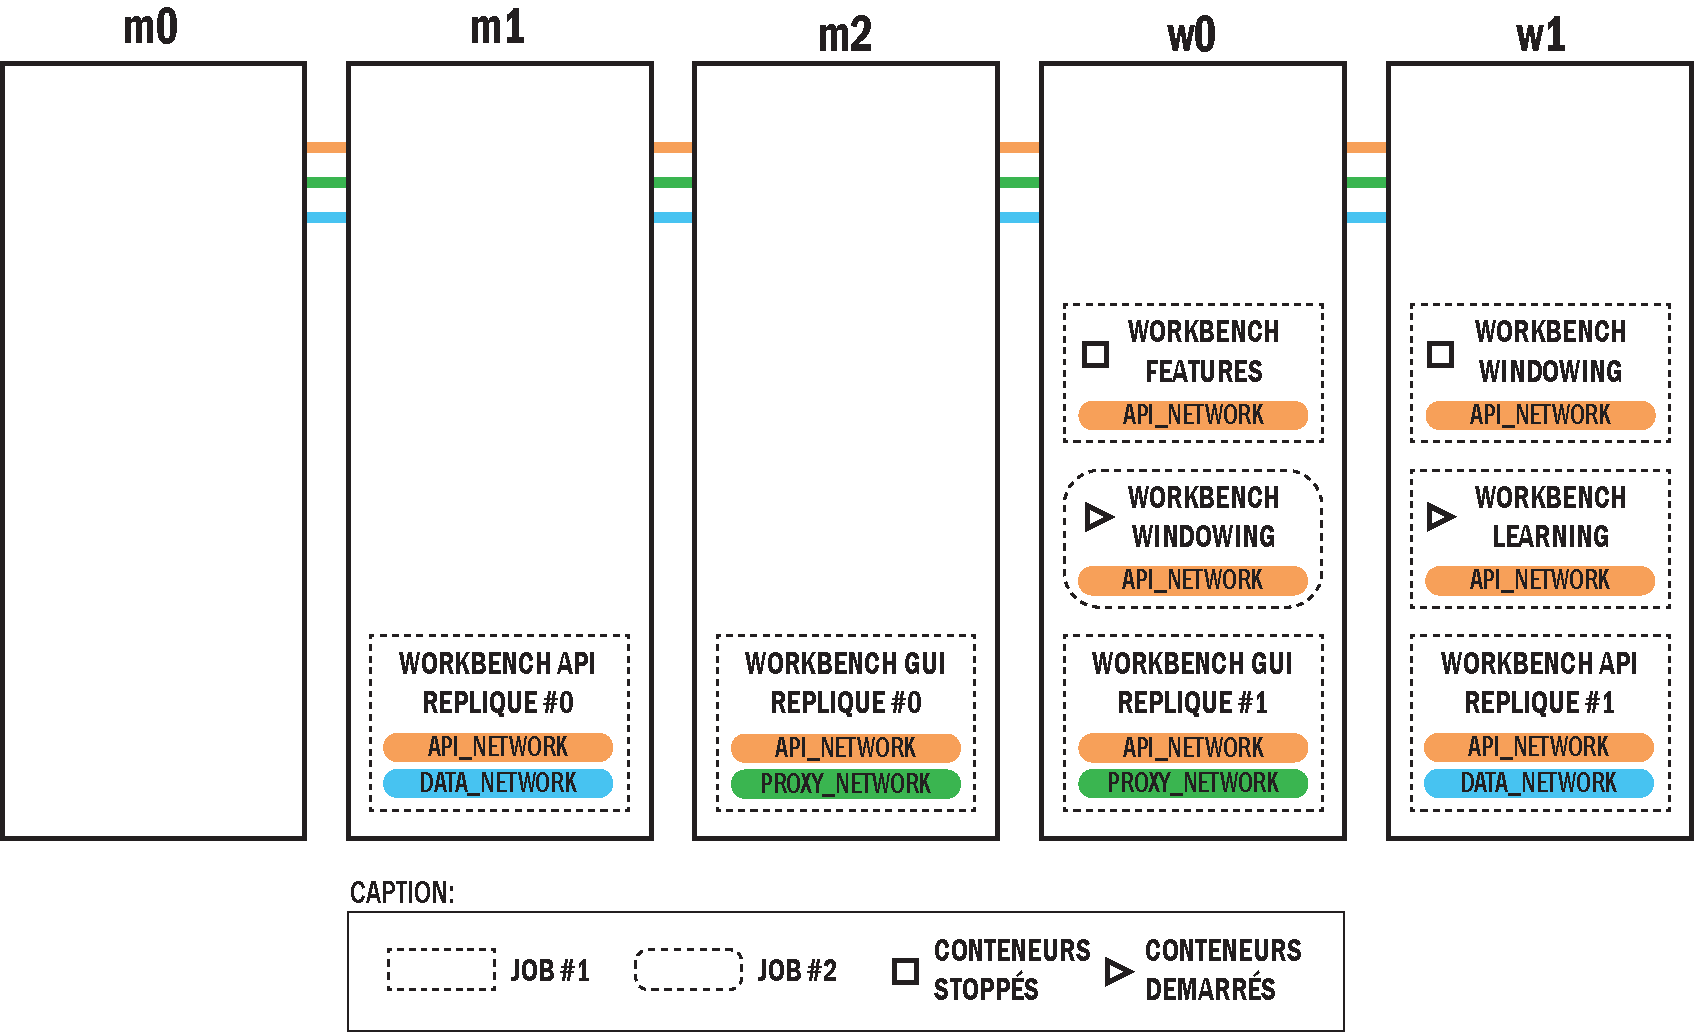
\includegraphics[width=.9\linewidth]{chapter6/containers_workbench.pdf}
        \caption{caption}
	\label{fig:containers_workbench}
\end{figure}

\subsection{API REST}

\begin{figure}[H]
	\centering
	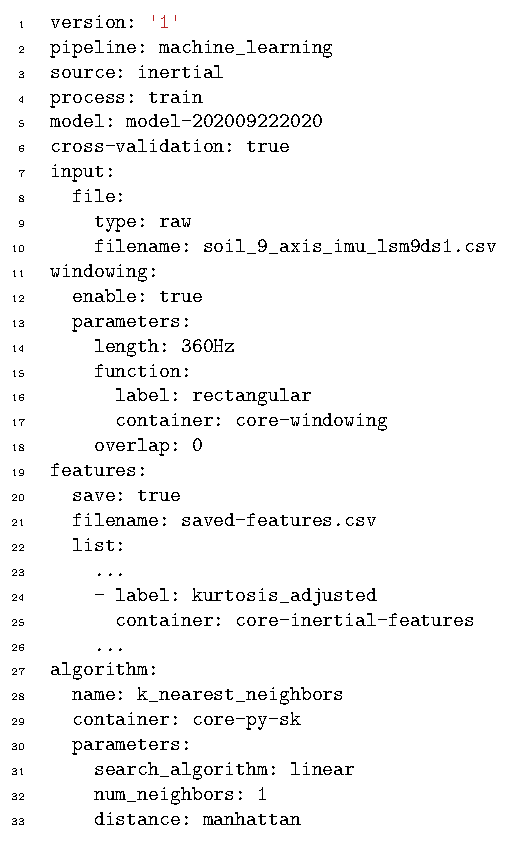
\includegraphics[width=.5\linewidth,keepaspectratio]{chapter6/pipeline_conf.pdf}
        \caption{caption}
	\label{fig:pipeline_conf}
\end{figure}

\subsection{Application Web}

\begin{figure}[H]
	\centering
	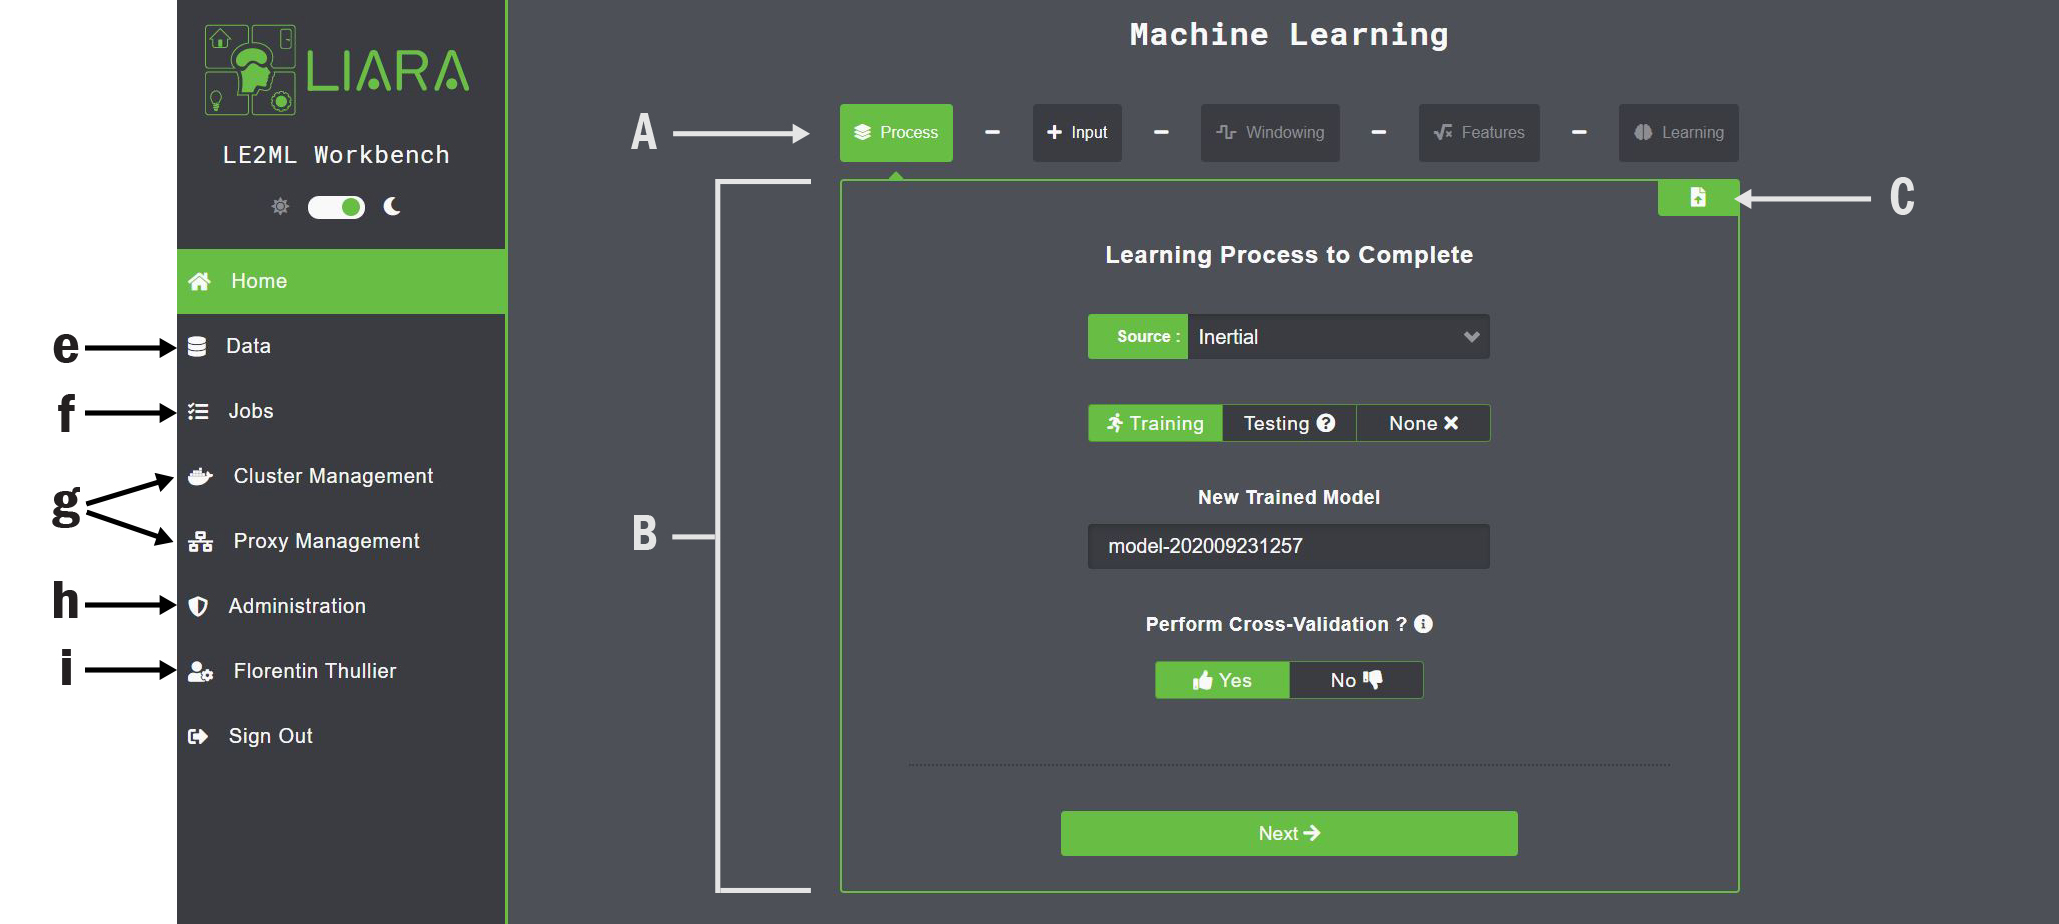
\includegraphics[angle=90,origin=c,height=\textwidth,keepaspectratio]{chapter6/le2ml_gui.jpg}
        \caption{caption}
	\label{fig:le2ml_gui}
\end{figure}

\subsection{Modules proposés}

\subsubsection{Fenêtrage}

\subsubsection{Extraction de caractéristiques}

\subsubsection{Apprentissage machine}

\section{Expérimentations \& Résultats}

\begin{table}[H]
    \centering
    \caption{caption.}
    \label{tab:previous_results}
    \begin{tabular}{@{}rccc@{}}
      \toprule
      \multicolumn{1}{l}{}              & \textit{Justesse}  &  $F\mbox{-} mesure$  & \textit{Kappa de Cohen}  \\ \midrule
      \textbf{$k$-NN}                   & 0.93               & 0.93                 & 0.89                     \\
      \textbf{\textit{Random Forest}}   & 0.92               & 0.92                 & 0.88                     \\ \bottomrule
    \end{tabular}
\end{table}

\begin{table}[H]
    \centering
    \caption{caption.}
    \label{tab:l2ml_results}
    \begin{tabular}{@{}rccc@{}}
      \toprule
      \multicolumn{1}{l}{}              & \textit{Justesse}  &  $F\mbox{-} mesure$  & \textit{Kappa de Cohen}  \\ \midrule
      \textbf{$k$-NN}                   & 0.91               & 0.91                 & 0.86                     \\
      \textbf{\textit{Random Forest}}   & 0.92               & 0.92                 & 0.88                     \\ \bottomrule
    \end{tabular}
\end{table}

\section{Conclusion}
